\documentclass[a4paper,12pt,fleqn]{article}

\usepackage[utf8]{inputenc}
\usepackage[T1]{fontenc}
\usepackage{graphicx}
\usepackage{anysize}
\usepackage{enumerate}
\usepackage{times}
\usepackage{amssymb}
\usepackage{amsmath}
\usepackage[polish]{babel}
%\marginsize{left}{right}{top}{bottom}
\marginsize{3cm}{3cm}{3cm}{3cm}
\sloppy
\bibliographystyle{abbrv}

\begin{document}
\bibliographystyle{abbrv}





Niech dana będzie funkcja ograniczona
{$f\!\colon\! [a,b]\to \mathbb {R}$} Sumą częściową (Riemanna) nazywa się liczbę
\[{R_{f,P(q_{1},\dots ,q_{n})}=\sum _{i=1}^{n}f(q_{i})\cdot \Delta p_{i}.}\]
Funkcję {$f$} nazywa się całkowalną w sensie Riemanna lub krótko R-całkowalną, jeśli dla 
dowolnego ciągu normalnego{$(P^{k})$} podziałów przedziału {$ [a,b],$}  istnieje (niezależna od wyboru punktów pośrednich) granica
\[R_{f}=\lim _{{k\to \infty }}R_{{f,P^{k}\left(q_{1}^{k},\dots ,q_{{n_{k}}}^{k}\right)}}\]
nazywana wtedy całką Riemanna tej funkcji. Równoważnie: jeżeli istnieje taka liczba {$R_{f},$}  że dla dowolnej liczby rzeczywistej {$\varepsilon >0$} istnieje taka liczba rzeczywista {$\delta >0,$} że dla dowolnego podziału {$ P(q_{1},\dots ,q_{n})$}  o średnicy {$ \mathrm {diam} \;P(q_{1},\dots ,q_{n})<\delta ;$}
	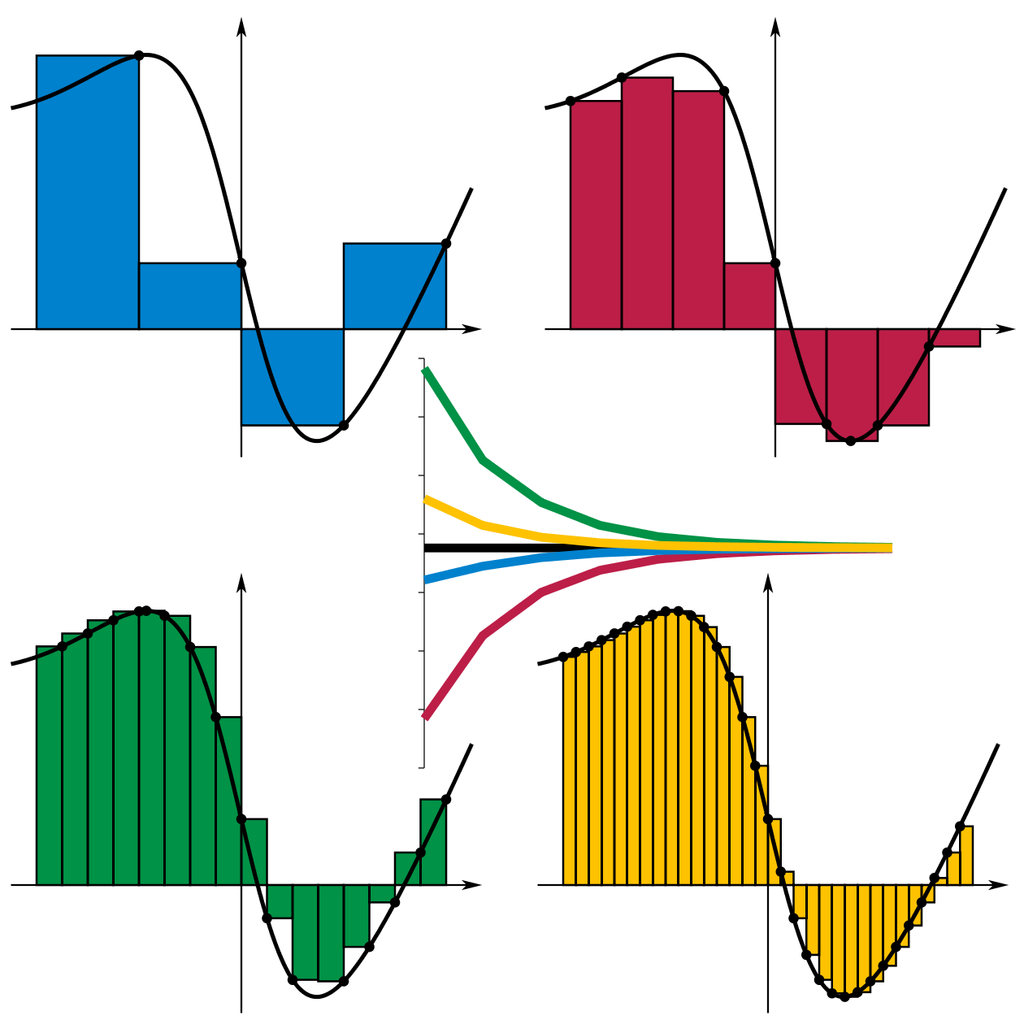
\includegraphics[width=0.48\textwidth]{Riem.png}
\end{document}
